\section{EppaBasic-ympäristö}
EppaBasicin tärkein tavoite on olla
helppo oppia,
mutta samalla mahdollistaa
monipuolisten ohjelmien toteuttamisen.
Yksinkertaiset ja helpot grafiikkakomennot ovat tärkeitä,
sillä moni aloitteleva (ja miksei myös kokenutkin)
ohjelmoija haluaa nähdä työnsä tulokset.

Toinen EppaBasicin tärkeä tavoite on,
että se on helppoa ottaa käyttöön.
Usein uutta ohjelmointikieltä käyttöön otettaessa
täytyy ladata ja asentaa useita ohjelmia,
jotka pitää vielä määrittää
toimimaan keskenään.
Monissa kouluissa
ongelmia saattaa lisäksi aiheuttaa byrokratia,
joka vaikeuttaa uusien ohjelmistojen asentamista
koulun tietokoneille.
EppaBasic onkin toteutettu
nettiselaimessa toimivaksi, joten
käyttöönotto onnistuu
helposti koneissa valmiiksi
olevilla ohjelmilla.

Ennen projektin aloittamista pohdimme,
täyttäisikö jokin olemassa oleva
kieli jo nämä tavoitteet.
Kuitenkin miettiessämme vaihtoehtoja
useat kielet olivat vanhentuneita,
niiden asentaminen tai oppiminen on hankalaa,
tai niillä grafiikan tekeminen on työlästä.
Tämän takia päädyimme uuden kielen tekemiseen.
Oman ohjelmointikielten luominen on lisäksi hauskaa
ja opettavaista.

\subsection{Käyttöliittymä}
\begin{figure}[h]
    \centering
    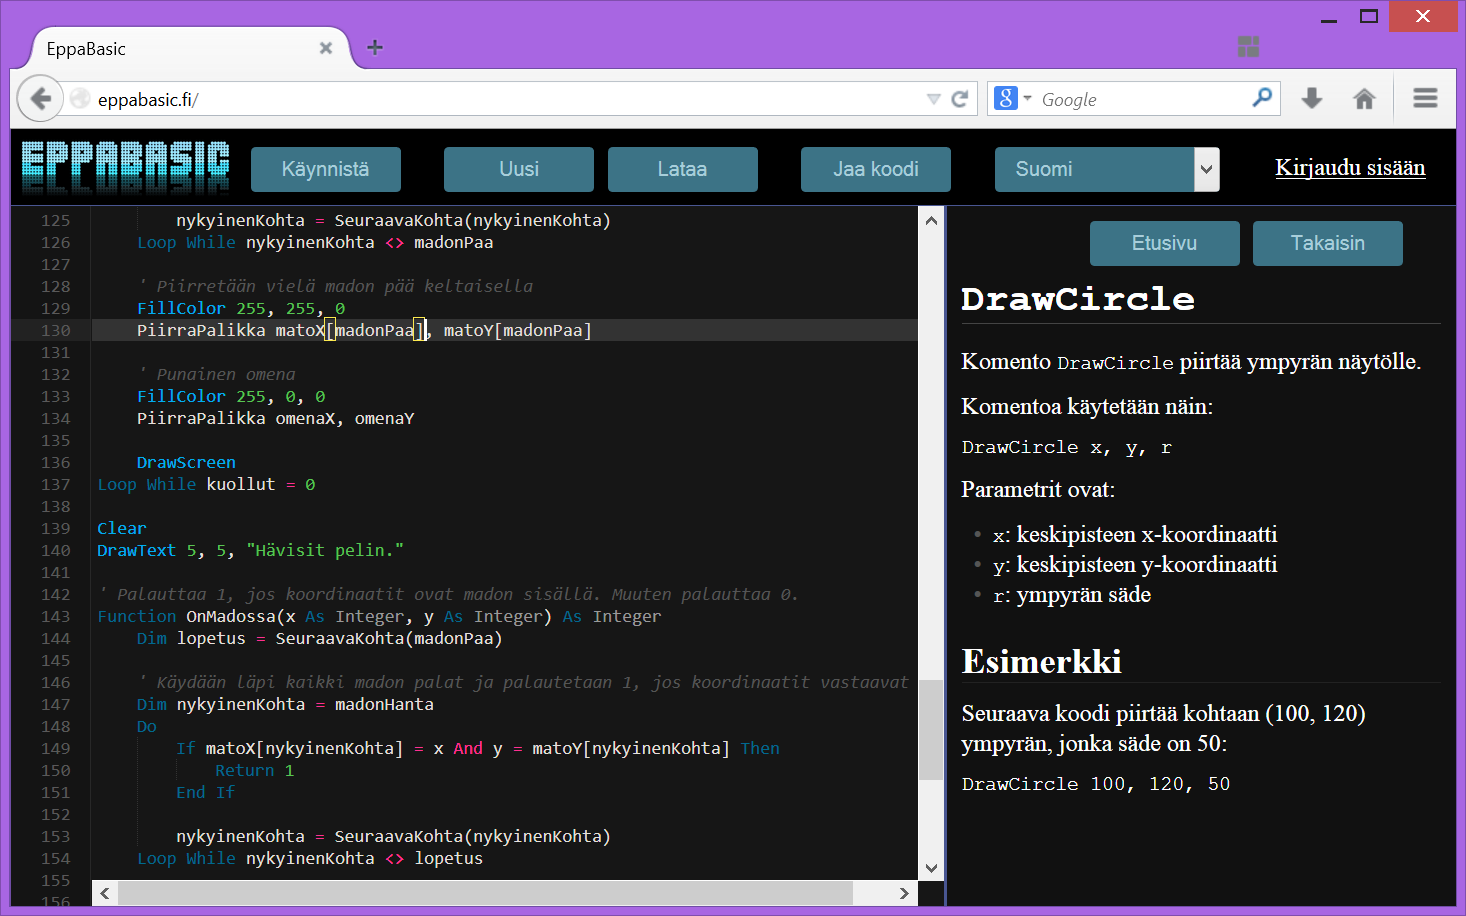
\includegraphics[width=1\textwidth]{kayttoliittyma}
    \caption{EppaBasicin käyttöliittymä. Ylhäällä työkalupalkki, vasemmalla koodimuokkain ja oikealla käyttöohje.}
    \label{img:kayttoliittyma}
\end{figure}

EppaBasicin käyttöliittymä on toteutettu
kokonaan käyttäen HTML:ää ja JavaScriptiä.
Näin on saatu aikaan kaikissa moderneissa
selaimissa toimiva yhtenäinen käyttöliittymä.

EppaBasicin käyttöliittymä tarjoaa kaikki
ohjelmointiin tarvittavat toiminnot.
Yläpalkissa on koodin suorittamisen käynnistävä
nappi sekä napit koodin tallentamiseen ja lataamiseen.
Lisäksi koodin voi jakaa muille käyttäjille linkin avulla.
Kirjautumalla sisään koodin voi tallentaa
omaan hakemistoon, jolloin se on käytettävissä
kaikilla tietokoneilla.

Käyttöliittymän vasemmalla reunalla on
koodimuokkain, johon
ohjelmakoodi kirjoitetaan.
Koodimuokkaimen oikealla puolella on
käyttöohje, jossa on kaikille
EppaBasicin funktioille
ja toiminnoille ohje esimerkkeineen.

EppaBasicin koodimuokkain mahdollistaa
virheiden ilmoittamisen käyttäjälle jo
koodia kirjoitettaessa.
Näin käyttäjä saa heti palautetta tekemistään
virheistä ja voi korjata ne saman tien.
Virhe sisältää käyttäjän oman
kielisen kuvauksen virheestä
(ks. Kuva \ref{img:virhe}).

\begin{figure}[h]
    \centering
    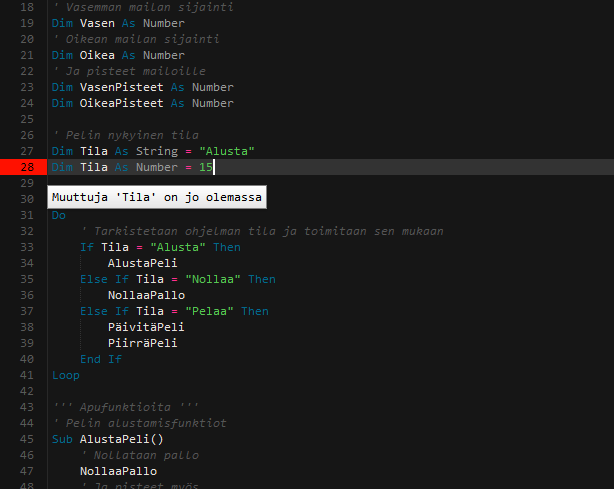
\includegraphics[width=0.5\textwidth]{virhe}
    \caption{EppaBasicin koodimuokkain, jossa näkyy käyttäjän tekemä virhe sekä virheen selitys.}
    \label{img:virhe}
\end{figure}

\subsection{Kieli}
EppaBasicin ohjelmointikieli tukee
muuttujia,
ehto- ja toistorakenteita,
matemaattisten lausekkeiden laskemista,
aliohjelmia, funktioita,
merkkijonoja ja
taulukoita.
EppaBasicissa on myös
laaja standardikirjasto,
jossa on matematiikka-,
merkkijono-, syöte- ja
grafiikkakomentoja.

Koodi \ref{code:geometria} näyttää,
miten EppaBasicilla voi piirtää
yksinkertaisia geometrisia muotoja.
Heittomerkin \eb{'} jälkeinen
teksti rivillä on kommenttia,
jota EppaBasic ei suorita.
Kommentit on tarkoitettu
työkaluksi ohjelmoijalle
koodin selkeyttämiseen.

\codeandimage{geometria}{Geometriaesimerkki}{code:geometria}

EppaBasicissa on
\eb{For}-toistorakenne, jonka
avulla voi suorittaa saman
koodin monta kertaa.
Toistettava koodi alkaa
\eb{For}-avainsanaa seuraavalta
riviltä ja loppuu ennen riviä,
jolla on \eb{Next}-avainsana.
\eb{For}-rakenteen sisällä voi
käyttää toistorakenteessa määriteltyä
muuttujaa, jonka arvo käy läpi
kaikki luvut annetulla välillä
(ks. Koodi \ref{code:for-geometria}).

\codeandimage{for-geometria}{Geometriaa \eb{For}-rakenteella}{code:for-geometria}

\eb{For}-toistorakennetta voi
käyttää myös matemaattisten 
ongelmien ratkausemiseen
(ks. Koodi \ref{code:for-summa}).

\codeandimage{for-summa}{Ohjelma, joka laskee summan $1^2+2^2+3^2+...+100^2$.}{code:for-summa}

EppaBasicilla tehdystä pelistä
esimerkkinä toimii
kielellä tehty moninpelattava
Pong-peli
(ks. Kuva \ref{img:pong}).
Pelin koodi on liitteessä \ref{app:pong}.
Peliä voi kokeilla myös
EppaBasicin sivustolla osoitteessa
\url{http://eppabasic.fi/#PONG}.

\begin{figure}[h]
    \centering
    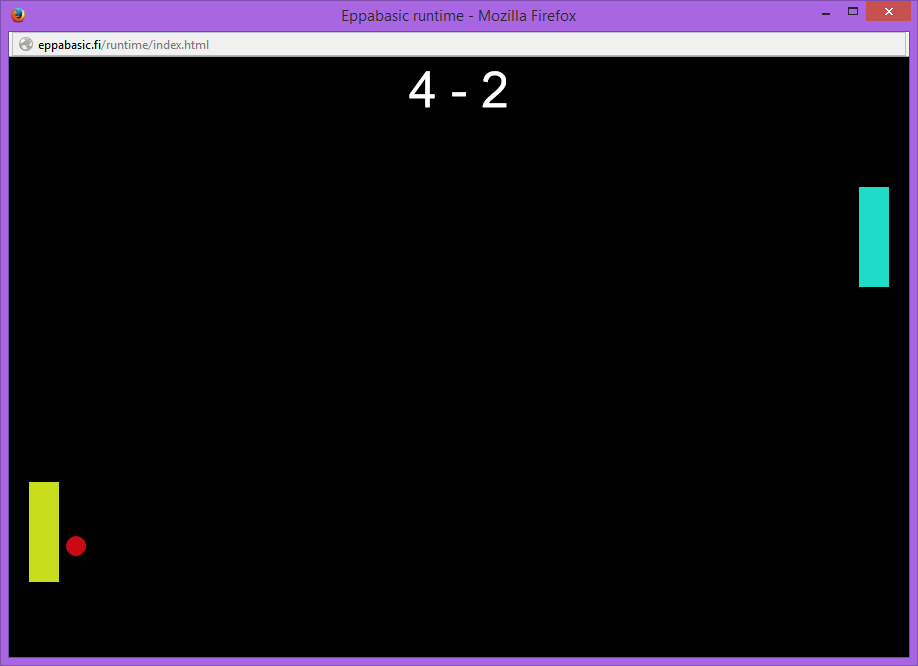
\includegraphics[width=0.5\textwidth]{pong}
    \caption{EppaBasicilla toteutettu kahdenpelattava Pong-peli.}
    \label{img:pong}
\end{figure}